\section{Introduction} \label{sec:introduction}
    \IEEEPARstart{R}{espiratory} motion reduces image resolution in \gls{PET} by introducing blurring \& mis-alignment artefacts~\cite{Nehmeh2008a}. 

\section{Methods} \label{sec:methods}
\subsection{Data Acquisition} \label{sec:data_acquisition}
        Seven dynamic \gls{FDG} acquisitions, with a \gls{FOV} covering the upper lung \& heart, were acquired on a \gls{GE} Discovery $710$. Each acquisition lasted approximately \SI{20}{\minute} with the acquisition starting before injection of the radiotracer. \gls{SS} were acquired in parallel using a \gls{RPM}.
        
    \subsection{Data Preparation} \label{sec:data_preparation}
        Data were unlisted into low resolution sinograms, at a time interval of \SI{500}{\milli\second}, using the \gls{GE} PetToolbox following~\cite{Bertolli2018Data-DrivenTomography}. Data was preprocessed by removing the first \& last element in the axial direction, this portion of the data contained significantly more noise than the rest of the data \& hinders later processes. Next, the data is normalised by finding its \gls{SSRB} normalisation factors \& applying those to it. Finally, the data initially has its mean subtracted, element by element, from it \& is then divided, element by element, before having a Freeman-Tukey transformation applied to stabilise the variance of the Poisson data. The Freeman-Tukey transformation is defined as:
        
        \begin{equation}
            S = 2 \sqrt{S + \frac{3}{8}}
        \end{equation}
        
        \noindent $S$ is the resultant sinogram of applying the Freeman-Tukey transformation to sinogram $S$~\cite{Freeman1950TransformationsRoot}.
    
    \subsection{Surrogate Signal Extraction} \label{sec:surrogate_signal_extraction}
        \subsubsection{Moving Window} \label{sec:moving_window}
            This method takes data from a window which initially starts as wide as one respiratory cycle but expands as the acquisition goes on \& applies \gls{PCA} to these windows independently. The motivation is that at early time points the variation caused by the tracer kinetics obscures that which comes from respiratory motion, however, if small enough time frames are taken, because of the different periods of the variation, of tracer kinetics \& respiratory motion, then the respiratory \gls{SS} should be obtainable. Specifically, after being gated into windows, which overlap by one half of the windows length, this data has a masked \gls{PCA} applied where the mask is a lower threshold which removes part of the noise. The \gls{SS} for each time point is then concatenated to the next using \gls{CC} to determine the sign of the \gls{SS}.
        
        \subsubsection{One \gls{PC}} \label{sec:one_pc}
            This method takes late time point \glss{PC} \& applies them to early time point data. The motivation is that the \glss{PC} of late time point data do not vary significantly. Therefore, it could be assumed that the variation of early time point \glss{PC} are caused mostly by the tracer kinetics. Specifically, this method takes the \gls{PC} from the last window of the moving window method~\Fref{sec:moving_window} \& multiplies it by the whole data set to acquire a \gls{SS} in one calculation.
        
        \subsubsection{Joint Method} \label{sec:joint_method}
            This method attempts to take the advantages of both the one \gls{PC} method as well as the static method, by truncating \& concatenating the result of the start of the one \gls{PC} method \& the end of the moving window method (where windows are long). The motivation is that the static method could be assumed to work better on static data \& once the tracer kinetics have subsided then the acquisition could be assumed to be static.
    
    
    \subsection{Evaluation} \label{sec:evaluation}
        To evaluate first the early time point \glss{SS} of one acquisition have been plotted alongside the \gls{RPM} \gls{SS} in order to visually assess the correlation of the \glss{SS}, additionally the \gls{CC} of the whole of each \gls{SS} of all acquisitions has also been calculated. Secondly, the \glss{SS} of one acquisition have been used to displacement gate the data from that acquisition into $10$ bins, reconstruct, \& then execute a \gls{MC} by registering (and applying a \gls{MM} using a linear regression over the \glss{DVF} \& \gls{SS}) the volumes to the mean position. Reconstructions were performed using \gls{GE} Duetto using \gls{TOF} \gls{OSEM} with two full iterations \& $24$ subsets.%~\cite{Hudson1994}.
        Volumes were post-filtered using a Gaussian blur with a kernel size of \SI{6.4}{\milli\metre} \gls{FWHM}. Comparisons between these \gls{MC} reconstructed volumes including: a visual analysis, a profile over the aorta (hot edge) \& \gls{SUV}\textsubscript{max}, \gls{SUV}\textsubscript{median} \& \gls{SUV}\textsubscript{peak}. \gls{SUV}\textsubscript{peak} here was defined following \gls{EANM} guidelines.%~\cite{Boellaard2015FDG2.0}
        
\section{Results} \label{sec:results}
    \begin{table}
        \centering
        \captionsetup{singlelinecheck=false, justification=centering}
        \caption{A comparison of the \gls{CC} between the \gls{RPM} \gls{SS} \& the \gls{SS} from the static \gls{PCA}, the moving window, the one \gls{PC} \& the joint methods for $7$ dynamic \gls{FDG} acquisition acquired on a \gls{GE} Discovery 710 \gls{PET}/\gls{CT} scanner.}
        
        \resizebox*{0.75\linewidth}{!}
        {
            \begin{tabular}{||c|cccc||}
                \hline
                \textbf{\gls{CC}} & \textbf{Static \gls{PCA}} & \textbf{Moving Window} & \textbf{One \gls{PC}} & \textbf{Joint Method} \\
                \hline
                \textbf{Acquisition $1$}   & $0.0387$  & $0.486$  & $0.565$  & $0.493$   \\
                \textbf{Acquisition $2$}   & $0.0985$  & $0.0361$ & $0.281$  & $0.0227$  \\
                \textbf{Acquisition $3$}   & $0.00797$ & $0.0388$ & $0.224$  & $0.00459$ \\
                \textbf{Acquisition $4$}   & $0.242$   & $0.0467$ & $0.273$  & $0.0946$  \\
                \textbf{Acquisition $5$}   & $0.0759$  & $0.793$  & $0.819$  & $0.798$   \\
                \textbf{Acquisition $6$}   & $0.0594$  & $0.246$  & $0.363$  & $0.259$   \\
                \textbf{Acquisition $7$}   & $0.160$   & $0.629$  & $0.203$  & $0.526$   \\
                \hline
            \end{tabular}
        }
        \label{tab:cross_correlation}
    \end{table}
    
    A comparison of \gls{CC} can be seen in in~\Fref{tab:cross_correlation}. The results for the moving window method show that it usually performs better than static \gls{PCA}, a reason why these results may be so varied is because the hyper parameters for this method were optimised for one acquisition \& as such results for other acquisitions may suffer. The results for the one \gls{PC} method are consistently better than the static \gls{PCA} method.
    
    \begin{figure}
        \centering
        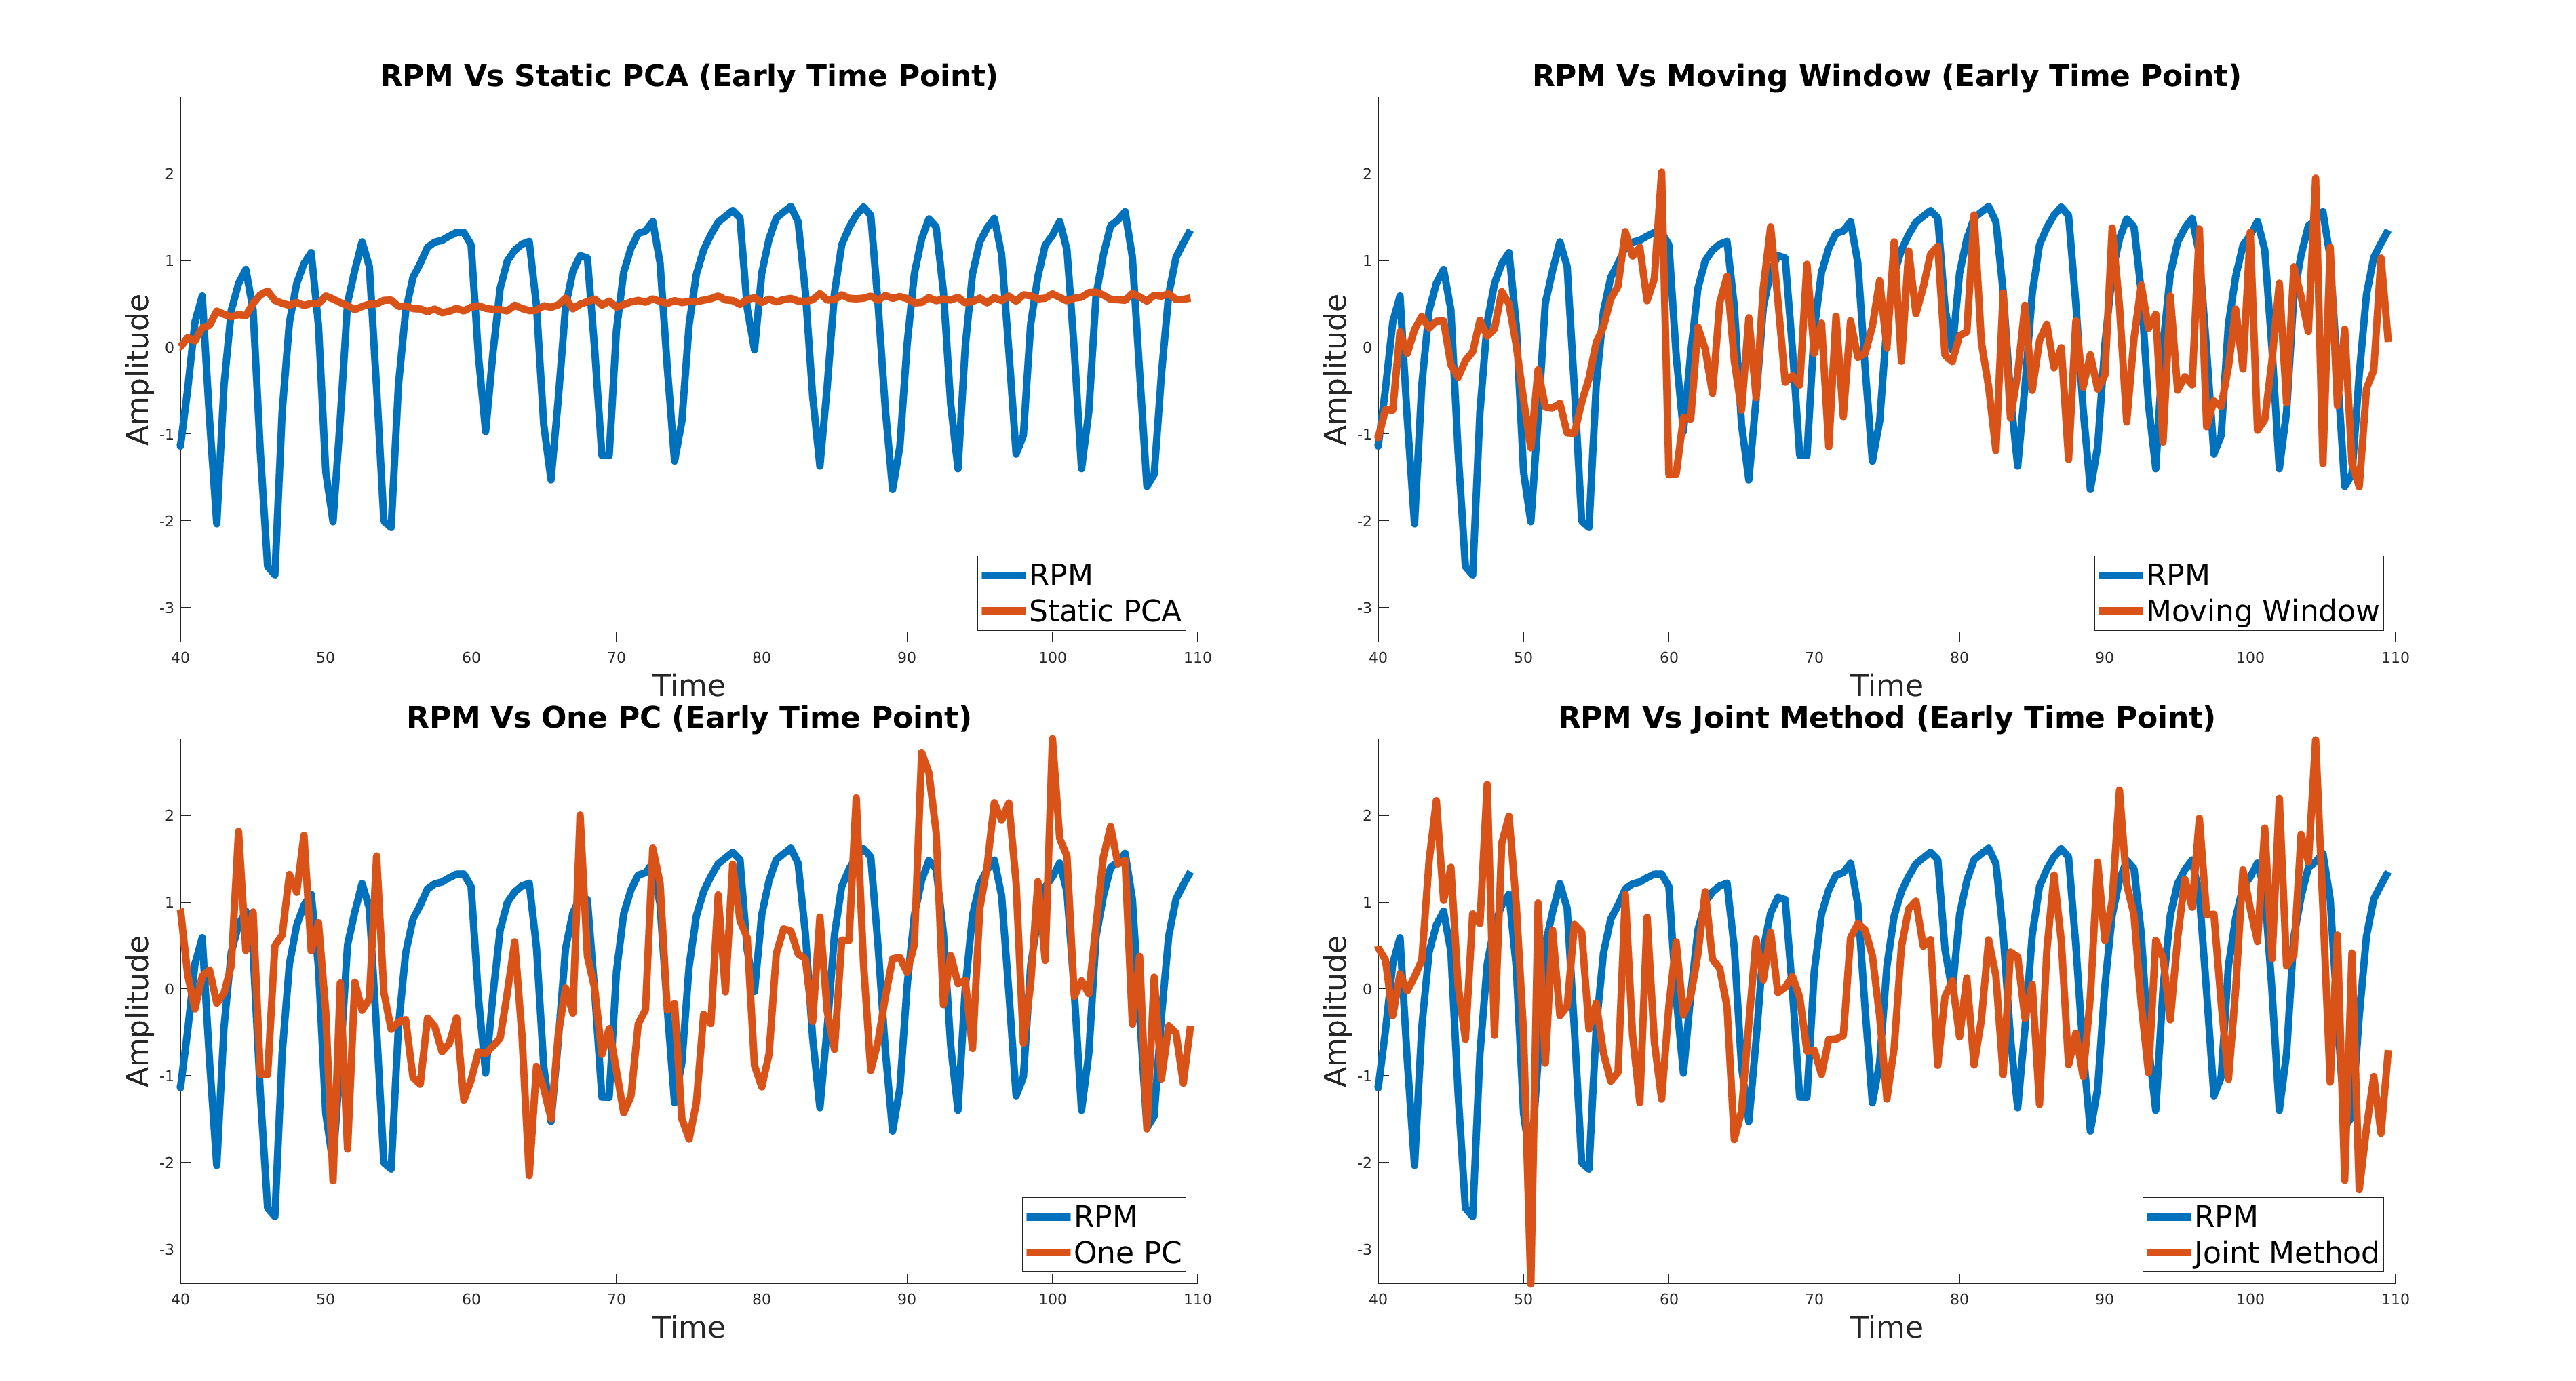
\includegraphics[width=1.0\linewidth]{figures/surrogate_signal.png}
        \captionsetup{singlelinecheck=false, justification=centering}
        \caption{A comparison between the \gls{RPM} \gls{SS} \& the \gls{SS} from the static \gls{PCA}, the moving window, the one \gls{PC} \& the joint methods for dynamic acquisition $1$ between \SI{40}{\second} \& \SI{110}{\second}.}
        \label{fig:surrogate_signal}
    \end{figure}
    
    \begin{figure}
        \centering
        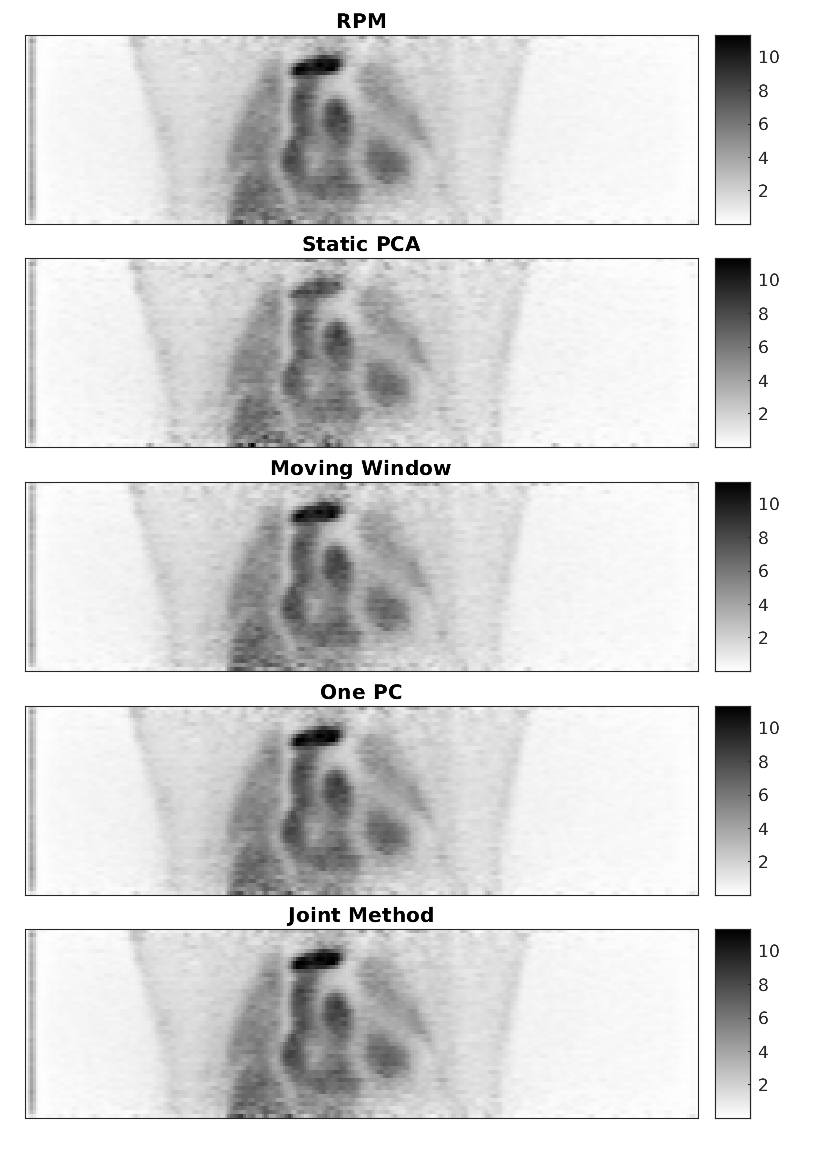
\includegraphics[width=0.75\linewidth]{figures/visual_analysis_pca.png}
        \captionsetup{singlelinecheck=false, justification=centering}
        \caption{Reconstructions of acquisition $1$ using \gls{MC} including the \gls{SS} derived from; first row: \gls{RPM}, second row: Static \gls{PCA} method, third row: moving window method, forth row: one \gls{PC} method \& firth row: joint method. Colour map ranges are consistent for all images.}
        \label{fig:visual_analysis}
    \end{figure}
    
    \begin{figure}
        \centering
        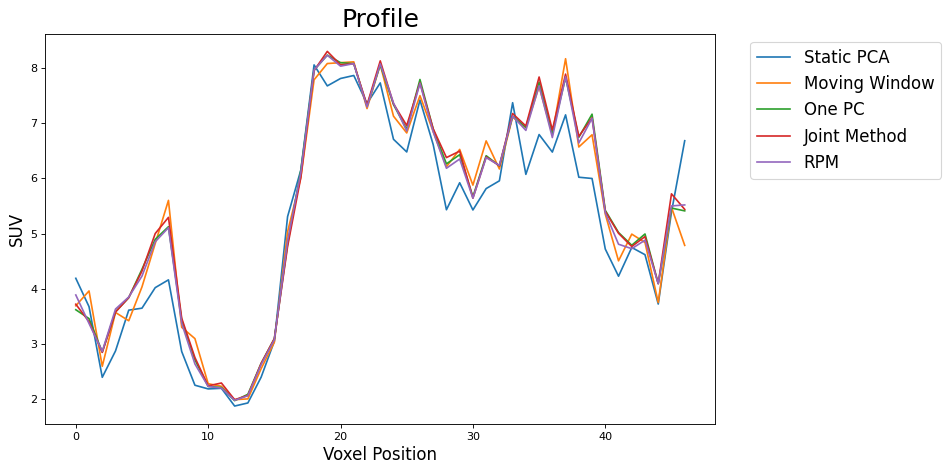
\includegraphics[width=0.5\linewidth]{figures/profile_pca.png}
        \captionsetup{singlelinecheck=false, justification=centering}
        \caption{A profile across the aeorta for reconstructions of acquisition $1$ using \gls{MC} including the \gls{SS} derived from; \gls{RPM}, Static \gls{PCA} method, moving window method, one \gls{PC} method \& joint method.}
        \label{fig:profile}
    \end{figure}
    
    \begin{table}
        \centering
        \captionsetup{singlelinecheck=false, justification=centering}
        \caption{Comparison of \gls{SUV}\textsubscript{max}, \gls{SUV}\textsubscript{median} \& \gls{SUV}\textsubscript{peak} between reconstructions of acquisition $1$ using \gls{MC} including the \gls{SS} derived from; \gls{RPM}, Static \gls{PCA} method, moving window method, one \gls{PC} method \& joint method.}
        
        \resizebox*{0.5\linewidth}{!}
        {
            \begin{tabular}{||c|ccc||}
                \hline
                \textbf{\gls{SUV}} & \textbf{Max} & \textbf{Median} & \textbf{Peak} \\
                \hline
                \textbf{\gls{RPM}}          & $18.4$ & $10.9$ & $12.6$ \\
                \hline
                \textbf{Static \gls{PCA}}   & $12.8$ & $10.6$ & $11.4$ \\
                \textbf{Moving Window}      & $14.5$ & $10.6$ & $11.3$ \\
                \textbf{One \gls{PC}}       & $18.5$ & $10.9$ & $12.6$ \\
                \textbf{Joint Method}       & $18.5$ & $11.0$ & $12.8$ \\
                \hline
            \end{tabular}
        }
        \label{tab:suv}
    \end{table}
    
    A plot of the \gls{SS} for all methods can be seen in~\Fref{fig:surrogate_signal}, the one \gls{PC} method matches the \gls{RPM} best in this example. The reconstructed data, using \glss{SS} from all methods can be seen in~\Fref{fig:visual_analysis}. The clarity of the reconstruction around the aorta seems diminished in the static \gls{PCA} example, it is similar in all other examples. A profile across the aorta can be seen in~\Fref{fig:profile}, this shows that the static \gls{PCA} method differs in its distribution compared to the others. \gls{SUV} results can be seen in~\Fref{tab:suv} \& show that \glss{SUV} are consistent with \gls{RPM} for both the one \gls{PC} method and the joint method.
    
\section{Discussion \& Conclusions} \label{sec:discussion_and_conclusions}
    
